		\section{Nombre: Viento temporal}\label{obs.vientoT}
	\subsection{Descripción}
	Ráfaga de viento. Impulsa al jugador de manera horizontal, dependiendo del nivel lo empujara hacia la izquierda o hacia la derecha. Su efecto no es constante, se activa y desactiva de manera periódica estando activo durante un tiempo determinado y desactivándose por otro tiempo determinado; los tiempos de actividad e inactividad pueden no ser los mismos. Para superar este obstáculo el jugador deberá aprovechar los tiempos de inactividad y cruzar la zona donde aparece la ráfaga.
	\subsection{Esquema}
Ver figura \ref{fig:vientoT}.
	\begin{figure}
  \centering
  \subfigure[La ráfaga de viento se activa durante un periodo determinado.]{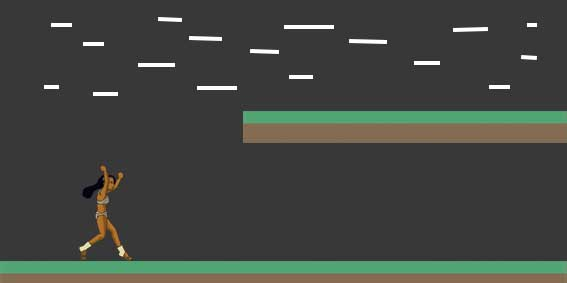
\includegraphics[width=0.3 \textwidth]{Imagenes/viento01}}
   \subfigure[La ráfaga de viento se desactiva durante un periodo determinado.]{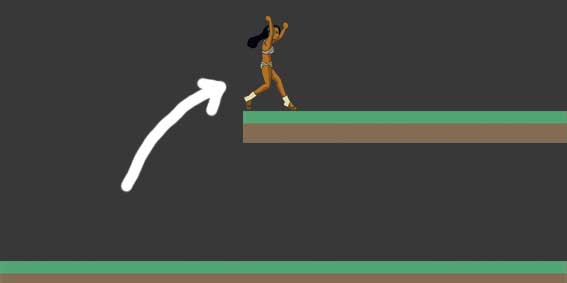
\includegraphics[width=0.3 \textwidth]{Imagenes/viento02}}
   \subfigure[La ráfaga de viento se vuelve a activar. Al hacer contacto con el jugador lo arrastra hacia la dirección en la que se mueve la ráfaga de viento.]{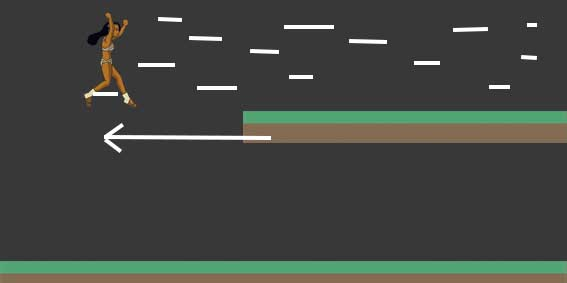
\includegraphics[width=0.3 \textwidth]{Imagenes/viento03}}
  \caption{Plataforma que cae.}
  \label{fig:vientoT}
\end{figure} 